\subsection{Кассовый компьютер (Устройство с дисплеем и клавиатурой)}

\begin{itemize}	
	\item Не вводятся цифры.
	Решение:
	\begin{myquote}
		Нажать клавишу NumLock (третья слева в нижнем ряду)
	\end{myquote}
\end{itemize}	
\subsection{Сканер штрихкодов}	
	\begin{itemize}	
		\item Перестал сканировать сканер (пищит и не сканирует).
		Решение :
		\begin{myquote}
			Обратиться по телефону в техподдержку для перезапуска сеанса работы с программой.
		\end{myquote}
\end{itemize}	    

\subsection{Фискальный регистратор}	
\begin{enumerate}	
	\item Чек не вышел, 1С показало ошибку связи с фискальным устройством (Error: Connection refuse, чек не напечатан и прочее).
	\item Фискальный регистратор не пробивает чек, не открывается или не закрывается смена.
	\item <<1С висит>>, крутится кружок, ничего не нажимается или вообще фискальник ведет себя <<как-то не так>>.
	\par
	\textbf{Решение:}
	\begin{myquote}
		\begin{enumerate}[a.]	
			\item Выключить электропитание устройства с помощью кнопки (обычно она находится справа внизу).
			\begin{figure}[H]
				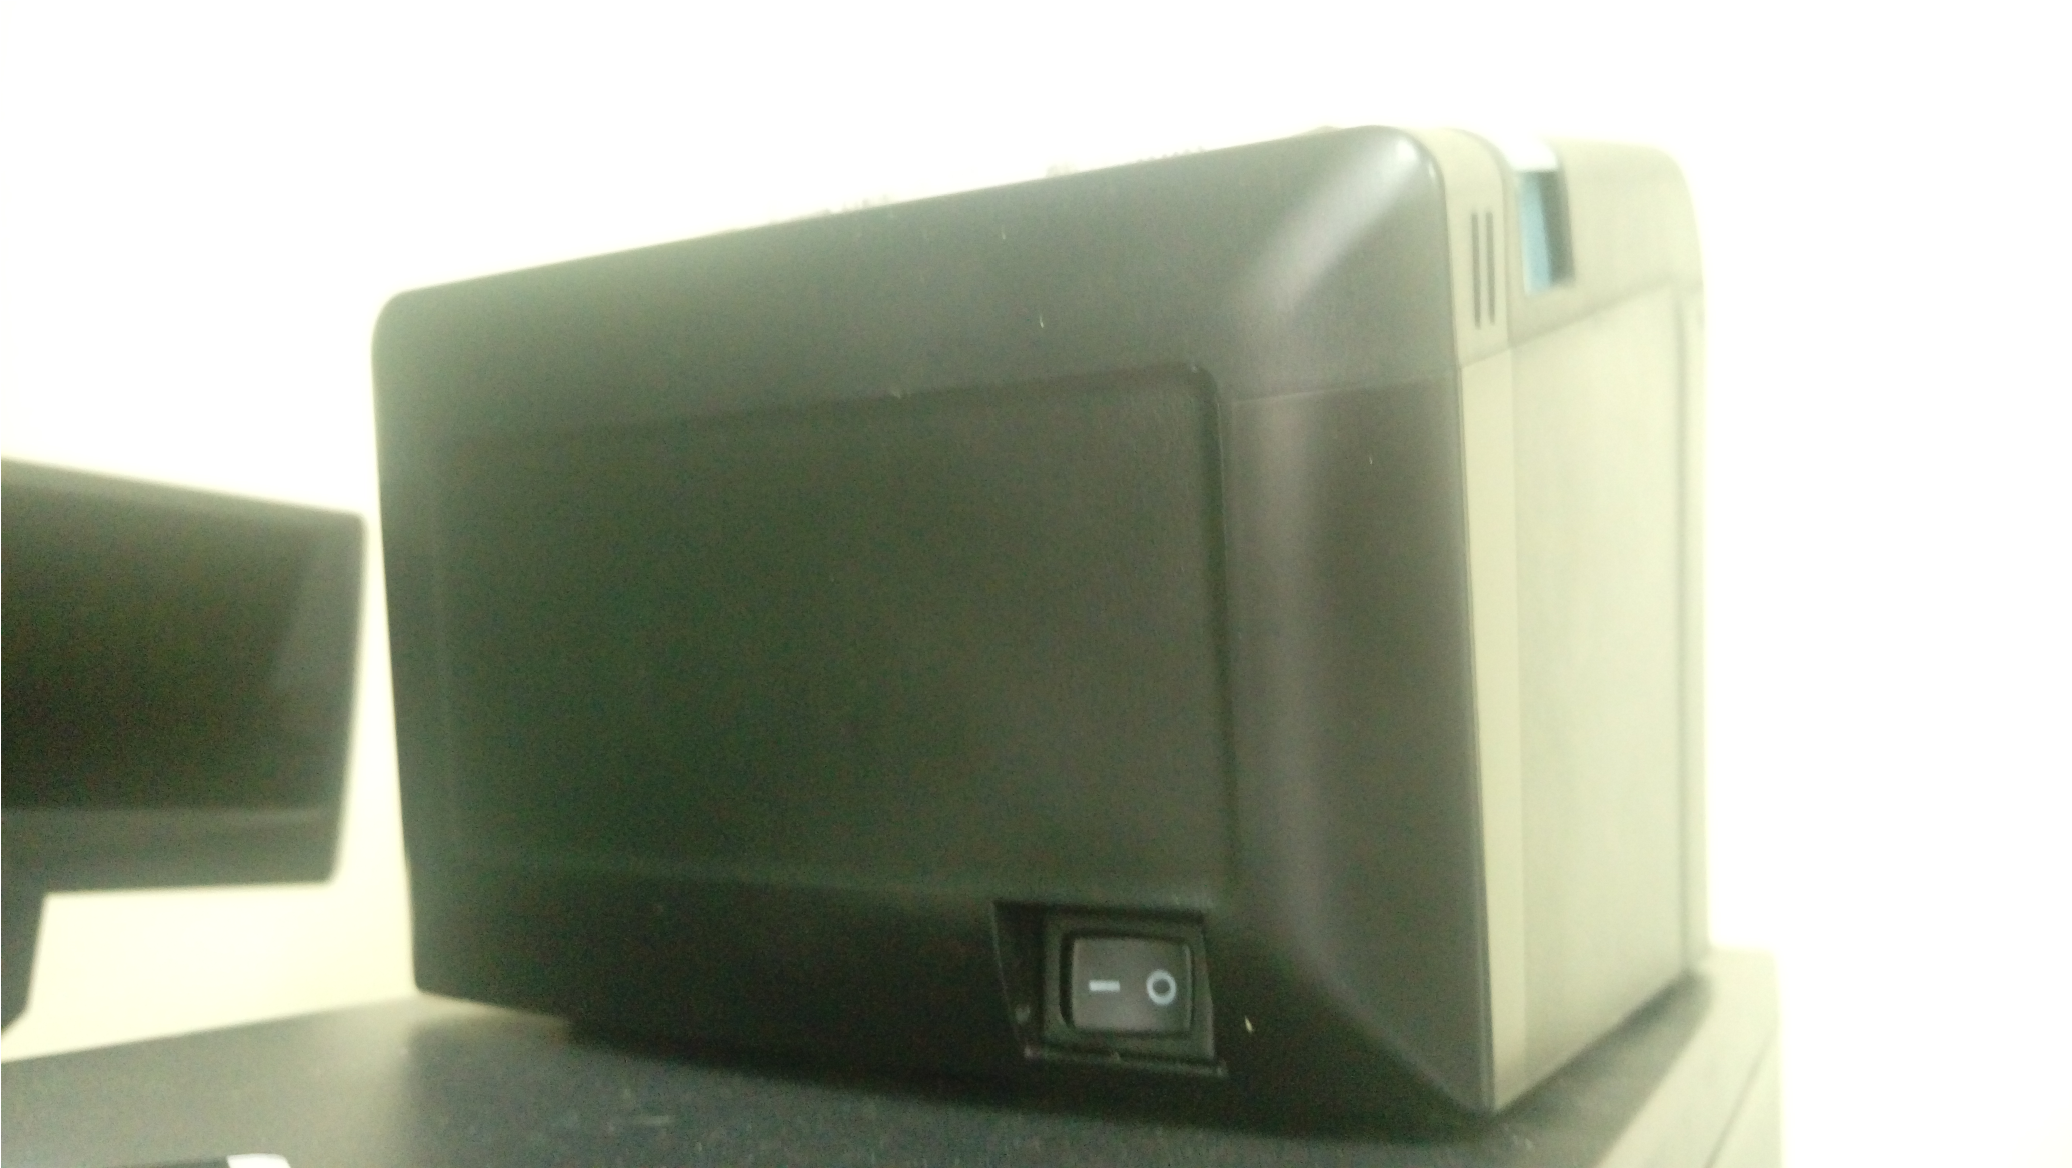
\includegraphics[width=0.7\textwidth]{15.png}
				\caption{Кнопка выключения}
				\label{ris:15.png}
			\end{figure}	
			\item Открыть бумажный лоток (ВНИМАНИЕ!!! Даже если Вы уверены, что бумага в фискальном регистраторе есть, всё равно лоток нужно открыть. Таким образом, мы устраняем <<виртуальное>>  замятие бумаги. Это обязательная процедура!).	
			\item Заново включить.					
			\item Провести оплату от клиента.
		\end{enumerate}	    	
	\end{myquote}
\end{enumerate}	    